\section{Astrocytic Networks}

The astrocytic contribution to conscious processing extends far beyond mere metabolic support of neuronal activity. Astrocytes form extensive networks through gap junctions, creating syncytia that span significant portions of neural tissue \cite{Giaume2010}. These syncytial networks serve as a parallel processing system that operates on slower timescales than neuronal circuits but provides crucial mechanisms for maintaining coherent conscious states.

Unlike neurons, which communicate primarily through discrete synaptic events, astrocytic syncytia enable direct cytoplasmic continuity between cells, allowing for seamless sharing of ions, metabolites, and signaling molecules across extended spatial domains \cite{Nagy2000}. This continuous internal medium creates an ideal substrate for maintaining coherent energy states over longer timescales than typical neuronal interactions.

The astrocytic networks demonstrate remarkable sophistication in their spatial organization \cite{Oberheim2012}. These networks can span multiple cortical columns, creating continuous domains for ion and metabolite distribution that transcend traditional anatomical boundaries. Through this extensive connectivity, astrocytic syncytia enable coordination across broader spatial domains than possible through neuronal connections alone, while providing mechanisms for stabilizing coherent energy states across neural tissue.

Temporal integration through astrocytic networks occurs on a fundamentally different scale than neuronal processing \cite{Bazargani2016}. Operating on timescales of seconds rather than milliseconds, astrocytes generate calcium waves that propagate across the syncytial network, maintaining stable background states that help regulate neuronal activity. This slower processing provides a complementary mechanism to rapid neuronal signaling, enabling the maintenance of coherent states across longer temporal windows.

The metabolic regulation provided by astrocytic networks proves essential for conscious processing \cite{Verkhratsky2018}. These networks coordinate energy distribution across active neural populations, maintain ion homeostasis in the extracellular space, and regulate neurotransmitter levels at synapses. Through these mechanisms, astrocytic syncytia support efficient energy utilization while enabling sustained conscious processing across distributed neural populations.

The interaction between astrocytic networks and neuronal systems creates a multi-scale organization where fast neuronal signaling becomes embedded within slower, more stable astrocytic domains \cite{Halassa2010}. This arrangement provides several crucial advantages for maintaining conscious states. The slower astrocytic processes help maintain coherent background states, while the syncytial networks enable coordination across extended spatial domains. Direct sharing of resources through the syncytial network supports sustained activity, while the combination of fast neuronal and slow astrocytic processes enables dynamic yet stable conscious states.

\begin{figure}[h]
    \centering
    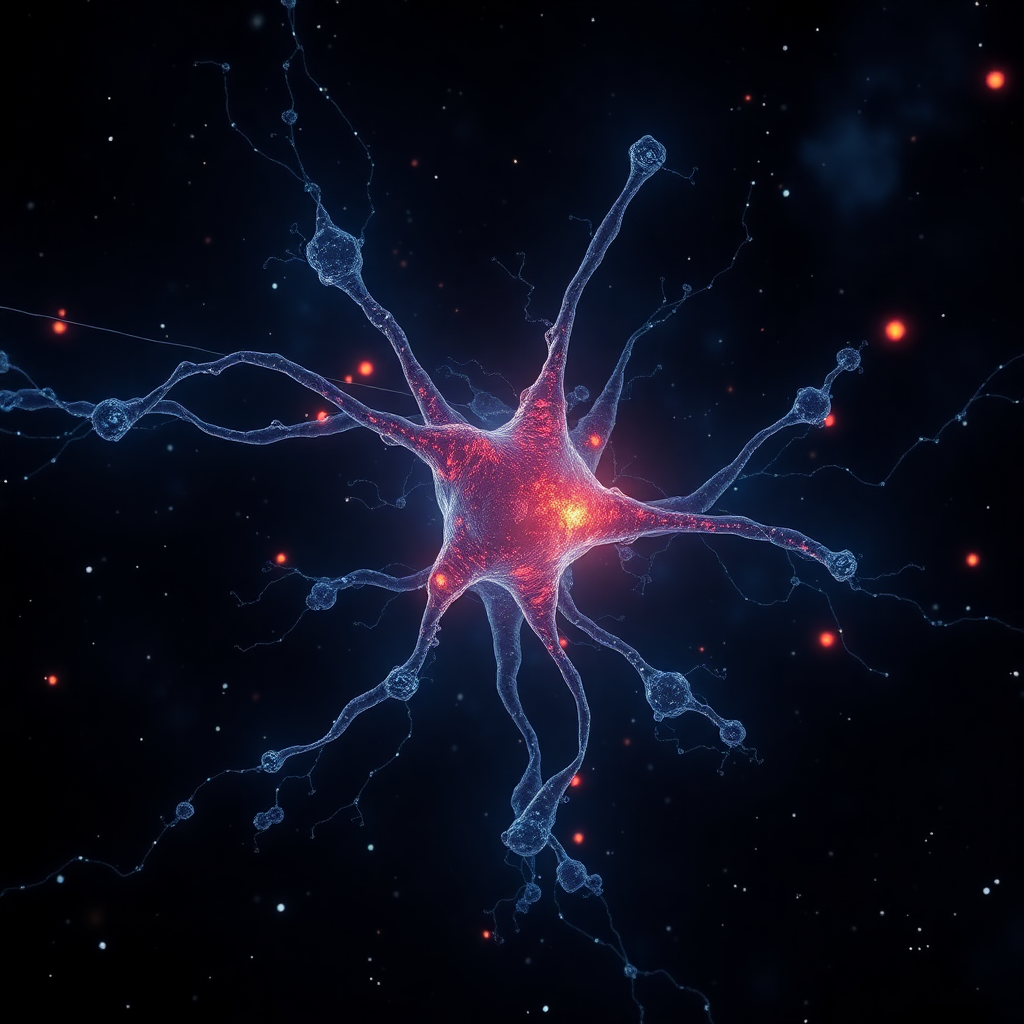
\includegraphics[width=0.8\textwidth]{images/astrocyte.png}

    \caption{Typical astrocyte.}
\end{figure}

The remarkable capacity of astrocytic networks to maintain coherent states while enabling dynamic responses becomes particularly evident in their role as regulators of neural excitability. Through careful modulation of extracellular ion concentrations and neurotransmitter levels, astrocytes help establish the precise conditions necessary for stable neural processing \cite{Araque2014}. This regulatory function extends beyond simple homeostasis to include active participation in information processing and state transitions.

Calcium signaling within astrocytic networks deserves particular attention \cite{Bazargani2016}. Unlike the rapid electrical signaling of neurons, astrocytes communicate through complex patterns of calcium waves that propagate across the syncytial network. These calcium signals can integrate information over longer temporal windows than neuronal activity, providing a mechanism for maintaining coherent states across extended periods. The patterns of calcium wave propagation reflect both local neural activity and broader network states, creating a sophisticated system for coordinating neural responses across multiple spatial and temporal scales.

The relationship between astrocytic networks and brain waves reveals another crucial aspect of conscious processing. Astrocytes help establish the conditions necessary for coherent oscillatory activity while modulating the spread of these oscillations through neural tissue \cite{Volterra2005}. Through regulation of extracellular ion concentrations and neurotransmitter dynamics, astrocytic networks can influence both the generation and propagation of brain waves. This interaction creates a feedback system where neuronal oscillations and astrocytic signaling work together to maintain stable patterns of conscious activity.

Gap junctions between astrocytes play an essential role in establishing the syncytial properties that enable coherent state maintenance \cite{Wallraff2006}. These direct cellular connections allow for rapid sharing of ions, metabolites, and small signaling molecules across extended spatial domains. The density and distribution of gap junctions can be dynamically regulated, providing a mechanism for modulating the extent and strength of network coupling based on current physiological demands.

The relationship between astrocytic networks and neural metabolism reveals sophisticated mechanisms for maintaining conscious states \cite{Parpura2012}. Through their extensive processes, astrocytes form specialized contacts with both blood vessels and synapses, creating a distributed system for matching energy supply to neural demand. This arrangement enables precise control over local metabolic conditions while maintaining broader patterns of energy distribution across neural tissue.

The integration of astrocytic networks with other brain systems demonstrates how biological organization can achieve both stability and flexibility through coordinated cellular interactions \cite{Khakh2015}. The ability of astrocytes to monitor and modulate neural activity while maintaining coherent energy states across extended spatial domains provides essential mechanisms for conscious processing. This sophisticated arrangement allows the brain to maintain stable conscious states while remaining adaptable to changing environmental demands.

Perhaps most significantly, astrocytic networks demonstrate how consciousness emerges not from neuronal activity alone but from the coordinated interaction of multiple cellular systems \cite{Nedergaard2003}. The continuous, field-like properties of astrocytic syncytia complement the discrete signaling of neurons, creating a hybrid system capable of supporting both rapid information processing and stable state maintenance. This integration of different cellular mechanisms proves essential for understanding how conscious states arise from biological organization.

The remarkable efficiency of astrocytic networks in managing ion homeostasis illustrates fundamental principles of conscious processing \cite{Bellot-Saez2017}. Through sophisticated regulation of extracellular potassium and calcium levels, these networks maintain the precise ionic conditions necessary for reliable neural signaling while preventing pathological states of over-excitation. This homeostatic function represents more than simple buffering - it creates the stable background conditions required for coherent conscious processing.

The study of astrocytic networks thus reveals fundamental principles about how biological systems achieve conscious processing \cite{Giaume2010}. Through their unique properties and extensive connectivity, astrocytes help create the conditions necessary for consciousness while providing mechanisms for maintaining coherent states across multiple spatial and temporal scales. This understanding proves essential for any complete theory of consciousness and suggests new approaches to both treating disorders of consciousness and developing artificial conscious-like systems.

The implications extend beyond neuroscience to fundamental questions about how biological systems maintain coherent states across multiple scales of organization \cite{Khakh2015}. The remarkable sophistication of gap junction networks demonstrates how evolution has refined cellular coupling mechanisms to support both stable conscious states and flexible adaptation to changing conditions. This deeper appreciation of biological connectivity proves essential for any complete theory of consciousness.

Moving beyond cellular networks, we must now examine how the extracellular matrix provides crucial structural and functional support for conscious processing. This complex network of proteins and molecules outside cells creates specialized microenvironments that shape both energy flows and information processing in neural tissue.